\begin{figure}[b]
\centering
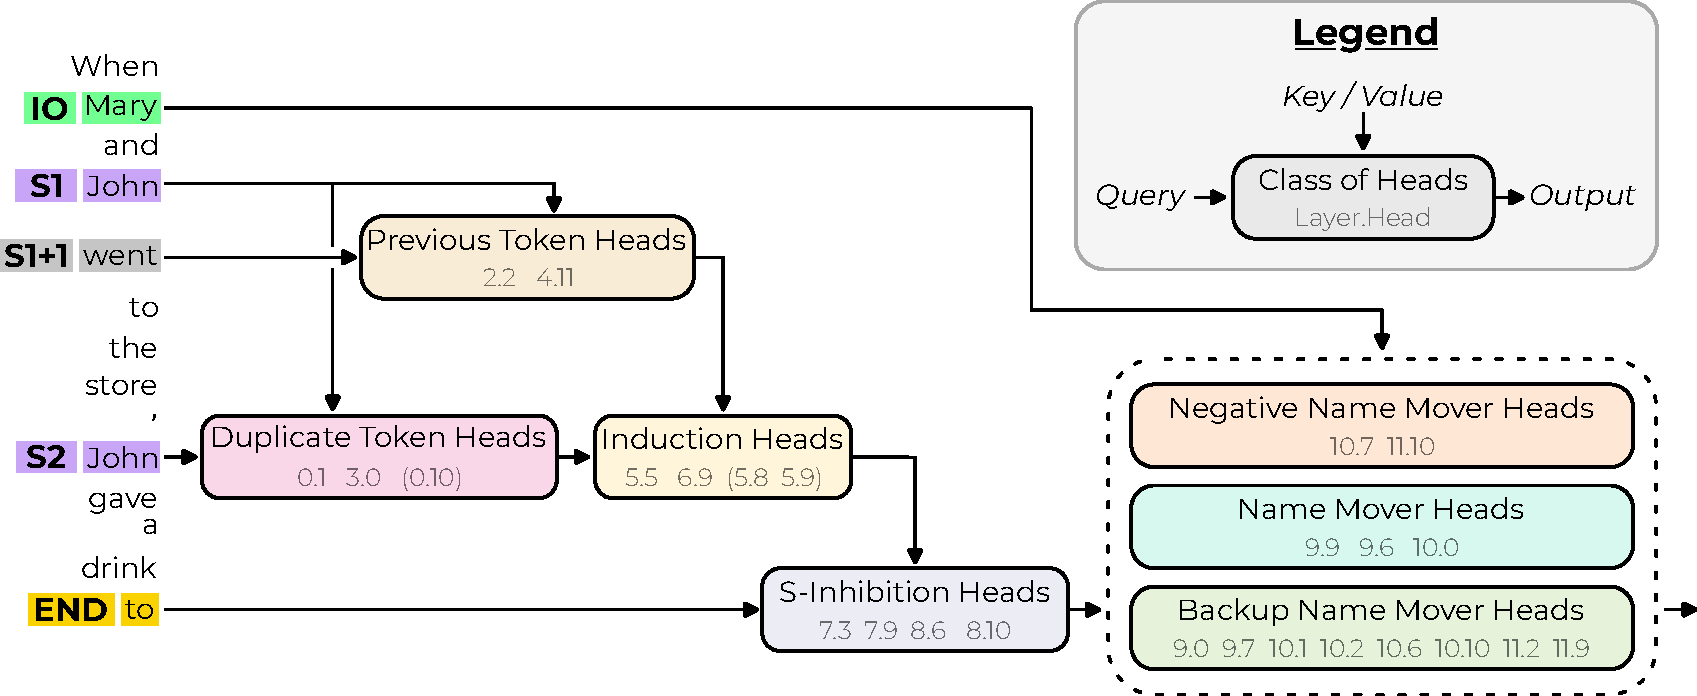
\includegraphics[width=0.8\textwidth]{figs/circuit_diag_v2.pdf}
\caption{We discover a circuit in GPT-2 small that implements IOI. The input tokens on the left are passed into the residual stream. Attention heads move information between residual streams: the query and output arrows show which residual streams they write to, and the key/value arrows show which residual streams they read from.}
% The most notable tokens are the IO token (the correct output for IOI), the S1 token (the subject of the first clause), the S2 token (the subject of the second clause) and the END token (the last token position). 
% , as shown in the `key/value' arrows: when different residual streams are attended to, a function of their input is written into the later residual stream.}
\label{fig:the_circuit}
\end{figure}

\section{Discovering the Circuit}
\label{sec:legibility}
%\subsection{Overview of the circuit}

\label{sec:overview}

We seek to explain how GPT-2 small implements the IOI task (Section \ref{sec:task_description}). Recall the example sentence ``When Mary and John went to the store, John gave a drink to". The following human-interpretable algorithm suffices to perform this task:
\begin{compactenum}
    \item Identify all previous names in the sentence (Mary, John, John).
    \item Remove all names that are duplicated (in the example above: John).
    \item Output the remaining name.
\end{compactenum}
% In this section, we will first describe the circuit in Figure~\ref{fig:the_circuit} in more detail, and then go through the steps needed to discover it. 
%width=0.8\textwidth, height = 4.9cm

%We claim that it is possible to partition a subset of GPT-2 small's heads into seven classes, each corresponding to a different function that the model uses to implement the IOI task. The major classes of heads are
Below we present a circuit that we claim implements this functionality.
Our circuit contains three major classes of heads, corresponding to the three steps of the algorithm above:
\begin{compactitem}
    \item \emph{Duplicate Token Heads} identify tokens that have already appeared in the sentence. They are active at the S2 token, attend primarily to the S1 token, and signal that token duplication has occurred by writing the position of the duplicate token.
    \item \emph{S-Inhibition Heads} remove duplicate tokens from Name Mover Heads' attention. They are active at the END token, attend to the S2 token, and write in the query of the Name Mover Heads, inhibiting their attention to S1 and S2 tokens.
    \item \emph{Name Mover Heads} output the remaining name. They are active at END, attend to previous names in the sentence, and copy the names they attend to. Due to the S-Inhibition Heads, they attend to the IO token over the S1 and S2 tokens. 
    % Their OV matrix is a name copying matrix, so in $\pioi$, they increase the logit of the IO token.
\end{compactitem}
A fourth major family of heads writes in the opposite direction of the Name Mover Heads, thus decreasing the confidence of the predictions. We speculate that these \emph{Negative Name Mover Heads} %are active at the END token and attend to the IO token preferentially, but write in the opposite direction (increasing S probability relative to IO). We speculate that these heads 
might help the model ``hedge'' so as to avoid high cross-entropy loss when making mistakes. %However, we do not fully understand their presence. %, but are not entirely sure why they are present. %Alternatively, they may be useful for other language tasks where names or other words are likely to be repeated several times, unlike in IOI.

There are also three minor classes of heads that perform related functions to the components above:

\begin{compactitem}
    \item \emph{Previous Token Heads} %are active at position S1+1, attend to token S, and 
    copy information about the token S to token S1+1, the token after S1. % into the residual stream.
    \item \emph{Induction Heads} perform the same role as the Duplicate Token Heads through an induction mechanism. They are active at position S2, attend to token S1+1 (mediated by the Previous Token Heads), and 
    %perform the same role as the duplicate-token heads, except that they they output a 
    their output is used both as a pointer to S1 and as a signal that S is duplicated.
    %interpreted as a signal that the S token previously appeared in the context. % \emph{the fact that the induction heads are copying} is a signal that $S2$ appeared previously, and should therefore be inhibited.
    \item Finally, \emph{Backup Name Mover Heads} do not normally move the IO token to the output, but take on this role if the regular Name Mover Heads are knocked out.
\end{compactitem}

% \todo{mention MLPs}
%Our circuit 
% we ignore MLPs
% In all our experiments, we never intervene on MLPs, they are always working in their natural state. Rigorously, this means our circuit also include them, even if their role is not understood.
In all of our experiments, we do not intervene on MLPs, %. They are treated as vital model components, like the 
layer norms,  or embedding matrices, focusing our investigation on understanding the attention heads. 
%Our circuit includes MLPs, despite the fact that we have not attributed semantic meaning to them.
%We do not study MLPs in this paper, so for simplicity our circuit also includes all the MLPs in GPT-2 small. 
%MLPs alone cannot process features across token position, thus we expect that the most interesting part of the behavior happen through attention heads. 
In initial investigations, we found that knocking out each MLP individually led to good task performance, except for the first layer. However, knocking out all MLPs after the first layer makes the model unable to perform the task (Appendix \ref{app:mlp}). A more precise investigation of the role of MLPs is left for future work.

Below we show how we discovered each of the seven components above, providing evidence that they behave as claimed. We found that it was easiest to uncover the circuit starting at the logits and working back step-by-step. Each step is divided into two parts. First, we trace the information flow backward from previously discovered components by finding attention heads that directly influence them; we do this using a technique we introduce called \emph{path patching}, which generalizes the application of causal mediation analysis to language models introduced in \citet{vig2020investigating}. Second, we characterize the newly identified heads by examining their attention patterns and performing experiments tailored to their hypothesized function. 


\subsection{Which heads directly affect the output? (Name Mover Heads)}
\label{sec:name movers} \label{sec:name_movers}
\label{sec:negative heads}

\textbf{Tracing back the information flow.} We begin by searching for attention heads $h$ directly affecting the model's logits. To differentiate indirect effect (where the influence of a component is mediated by another head) from direct effect, we designed a technique called \textbf{path patching} (Figure \ref{fig:directed_graph_figure}). 

% Two datasets are necessary for this technique: a target dataset containing the behavior to investigate (in our case, samples from $\pioi$) and a baseline dataset where the behavior is not present (in our case, samples from the $\pabc$ distribution introduced in Section \ref{sec:knockouts}). 
% %. It is a variation of $\pioi$ where the names are replaced by random names
% %This technique enable a comparative study of the model on two datasets: the target dataset (in our case $\pioi$) and a baseline where the IOI behavior is not present (in our case, the CDE distribution introduced in Section \ref{sec:knockouts}. It is a variation of $\pioi$ where the names are replaced by random names). 

% The experiment is divided into three steps. i) We run the model on the two datasets and save the outputs of all attention heads. ii) We rerun the model on the target dataset, but we \emph{patch}, or replace, the output of $h$ by its value on the baseline dataset. We do not recompute the output of the heads appearing in later layers than $h$, instead we freeze them so they have the same output as on the target dataset. Because all heads after $h$ are frozen, this can be seen as patching the path\footnote{We recompute MLPs along the path $h\to \text{Logits}$. This means that path patching involves solely the edges that are in the computational subgraph made of attention heads only. See Appendix \ref{app:path_patching} for full technical details on path patching.} $h\to \text{Logits}$ from the baseline dataset. iii)~We quantify the behavior on the IOI task by measuring the logit difference. 
Path patching replaces part of a model's forward pass with activations from a different input.
Given inputs $\xorig$ and $\xnew$, and a set of paths $\mathcal{P}$ emanating from a node $h$, path patching runs a forward pass on $\xorig$, but for the paths in $\mathcal{P}$
it replaces the activations for $h$ with those from $\xnew$. In our case, $h$ will be a fixed attention head
and $\mathcal{P}$ consists of all direct paths from $h$ to a set of components $R$, i.e. paths through residual connections
and MLPs (but not through other attention heads); this measures the counterfactual effect of $h$
on the members of $R$. The layers after the element from $R$ are recomputed as in a normal forward pass. See Appendix~\ref{app:path_patching} for full details of the method.  % for pseudocode

We will always take $\xorig$ to be a sample from $\pioi$, and $\xnew$ the corresponding
sample from $\pabc$ (i.e.~where the names in the sentence are replaced by three random names). We run
path patching on many random samples from $\pioi$ and measure how this affects the average logit difference. Pathways $h \to R$ that are critical to the model's computation should induce a large drop in logit difference when patched, since the $\pabc$ distribution removes the information needed to complete the IOI task.

To trace information back from the logits, we run path patching for the pathway $h \to \text{Logits}$ for each head $h$ at the END position and display the effect on logit difference in Figure \ref{fig:name_moversA}.
%We display the results of this experiment for every $h$ at the END position in Figure \ref{fig:name_moversA}. 
We see that only a few heads in the final layers cause a large effect on logit difference. Specifically, patching 9.6, 9.9, and 10.0 causes a large drop (they thus contribute positively to the logit difference), while 10.7 and 11.10 cause a large increase (they contribute negatively to the logit difference).

%$\lambda_{i, j}$ in Figure \ref{fig:name_moversA}. We see that only a few heads in the final layers have large logit projection $\lambda_{i, j}$. Specifically, 9.6, 9.9, and 10.0 have a large positive score, while 10.7 and 11.10 have a large negative score. 

%We begin by identifying which attention heads directly affect the model's output: in other words, the heads writing in the residual stream at the END position, in a direction that has high dot product with the logit difference.
%
% More 
%Formally, let $W_U$ denote the unembedding matrix, $\overline{\text{LN}}$ a layer norm operation (see Appendix \ref{app:layer_norm}) and $W_U[IO]$, $W_U[S]$ the corresponding unembedding vectors for the $IO$ and $S$ tokens. We searched for heads $(i, j)$ such that
%\begin{equation}
%\label{eq:proj1}
%    \lambda_{i, j} \eqdef \mathbb{E}_{X \sim \pioi}[\langle \overline{\text{LN}} \circ h_{i,j}(X), W_U[IO] - W_U[S] \rangle]
%\end{equation}
%had large magnitude. Recall that $h_{i, j}(X)$ is the value that head $(i, j)$ writes into the residual stream on input $X$. Therefore, heads with $\lambda_{i, j} > 0$ correctly promote the IO token over the S token (on average). The unembedding projection in (\ref{eq:proj1}) is called the \emph{logit lens} and has been used in previous work to interpret  intermediate activations \citep{LogitLens} and parameters \citep{dar2022analyzingEmbedSpace}. % in transformers.

%scaled by layer norm(see Appendix \ref{app:layer_norm})
%We display the values of $\lambda_{i, j}$ in Figure \ref{fig:name_moversA}. We see that only a few heads in the final layers have large logit projection $\lambda_{i, j}$. Specifically, 9.6, 9.9, and 10.0 have a large positive score, while 10.7 and 11.10 have a large negative score. 
% We next investigate these positive and negative heads in detail.

\textbf{Name Mover Heads.} To understand the heads positively influencing the logit difference, we first study their attention patterns. We find that they attend strongly to the IO token: the average attention probability of all heads over $\pioi$ is 0.59. We hypothesize that these heads (i) attend to the correct name and (ii) copy whatever they attend to. We therefore call these heads \emph{Name Mover Heads}. 

%Since attention patterns can be misleading \citep{attention_not_explanation}, we check whether attention is correlated with the heads' functionality. 

%\ac{See comment for edit of this paragraph} 
To verify our hypothesis, we design experiments to test the heads' functionality.
%Formally, 
Let $W_U$ denote the unembedding matrix, and $W_U[IO]$, $W_U[S]$ the corresponding unembedding vectors for the $IO$ and $S$ tokens. We scatter plot the attention probability against the logit score $\langle h_i(X), W_U[N]  \rangle$, measuring how much head $h_i$ on input $X$ is writing in the direction of the logit of the name $N$ (IO or S). The results are shown in Figure~\ref{fig:name_moversC}: higher attention probability on the IO or S token is correlated with higher output in the direction of the name (correlation $\rho>0.81$, $N=500$)\footnote{In GPT-2 small, there is a layer norm before the final unembedding matrix. This means that these dot products computed are not appropriately scaled. However, empirically we found that approaches to approximating the composition of attention head outputs with this layer norm were complicated, and resulted in similar correlation and scatter plots.}. 
% \ac{Appendix I explains the limitations of this attribution technique and verifies that our projection analysis reflects the true direct effect of attention heads.} %Based on this result, we hypothesize that these heads (i) attend to names and (ii) copy whatever they attend to. We therefore call these heads \emph{Name Mover Heads}. 

To check that the Name Mover Heads copy names generally, we studied what values are written via the heads' OV matrix. Specifically, we first obtained the state of the residual stream at the position of each name token after the first MLP layer. Then, we multiplied this by the OV matrix of a Name Mover Head (simulating what would happen if the head attended perfectly to that token), multiplied by the unembedding matrix, and applied the final layer norm to obtain logit probabilities. We compute the proportion of samples that contain the input name token in the top 5 logits ($N = 1000$) and call this the copy score. All three Name Mover Heads have a copy score above $95\%$, compared to less than $20\%$ for an average head.
% Let $L_0$ denote the first layer of the transformer, $W_{OV}^h$ the OV matrix for a head $h$, and $U$ the unembedding\footnote{Layer norm and then a linear map, see Appendix \ref{app:notation}}. Let $\text{Top}_5 : \mathbb{R}^V \to \{ 0, 1\}$ be the binary function that maps the $V$ logits to whether the IO is in the top 5 tokens. Then define the positive ($+$) and negative ($-$) copying scores as
% \begin{equation}
% \label{eq:proj2}
%     s_{\text{copy}}^\pm(h) \eqdef \mathbb{E}_{X \sim \pioi}[ \text{Top}_5( U \circ (\pm W_{OV}^h) \circ L_0 (X)) ]
% \end{equation}

% where we report the score as a percentage. We find that all three name-movers have a copy score above $95\%$ (compared to less than $20\%$ for an average head).

% ARTHUR READ THROUGH TILL HERE
\textbf{Negative Name Mover Heads.}
In Figure \ref{fig:name_moversB}, we also observed two heads causing a large increase, and thus negatively influencing the logit difference. We called these heads \emph{Negative Name Mover Heads}. These share all the same properties as Name Mover Heads except they (1) write in the opposite direction of names they attend to and (2) have a large \textit{negative} copy score--the copy score calculated with the negative of the OV matrix (98\% compared to 12\% for an average head).  %strongly in the direction of the S token. 

% \ref{fig:name_movers}

\begin{figure}
    \centering
    \hfill
     \begin{subfigure}[b]{0.20\textwidth}
         \centering
         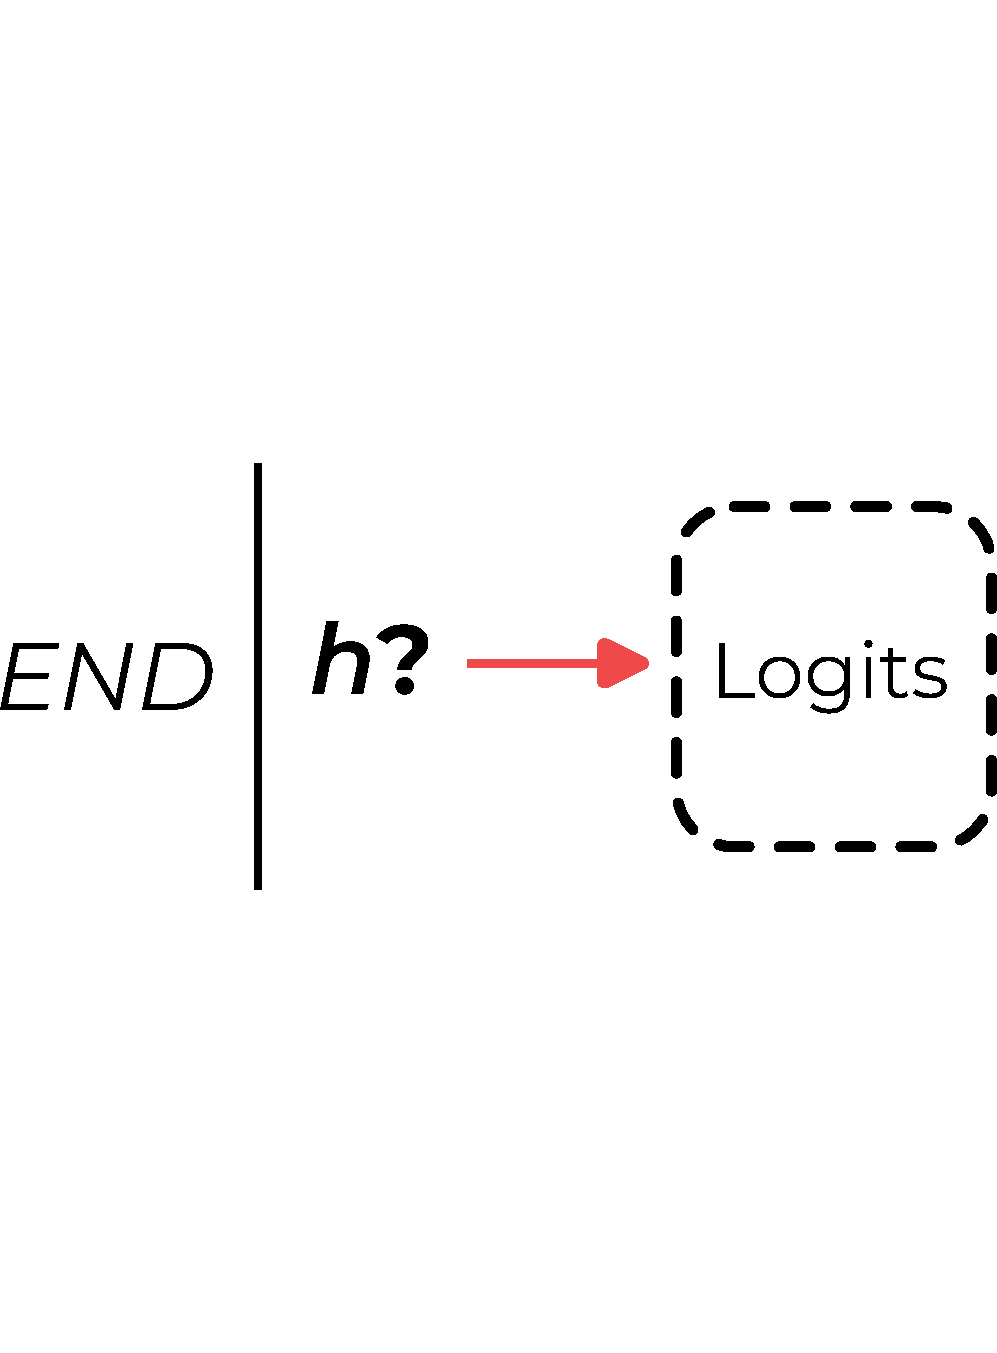
\includegraphics[width=\textwidth]{figs/fig_nm_neg_legibilityAA.pdf}
         \caption{}
         \label{fig:name_moversA}
     \end{subfigure}
     \hfill
     \begin{subfigure}[b]{0.30\textwidth}
         \centering
         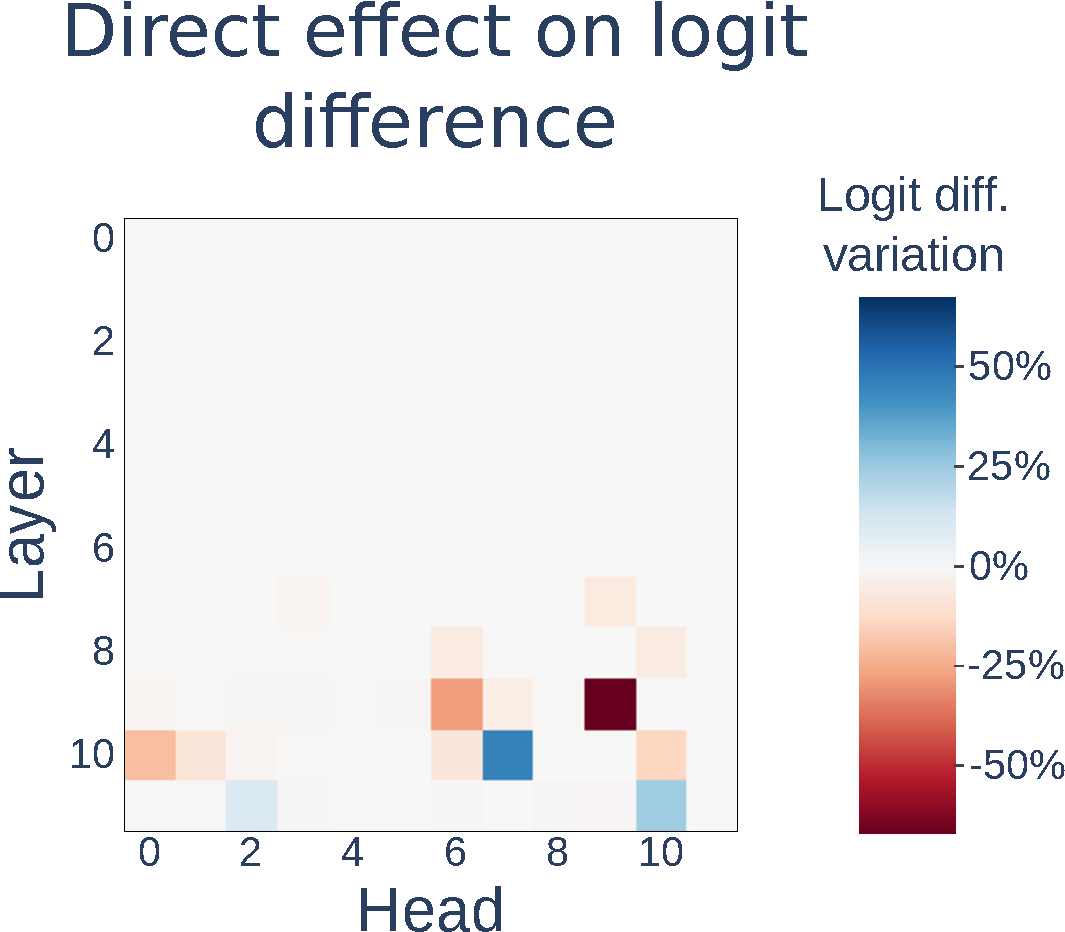
\includegraphics[width=\textwidth]{figs/fig_nm_neg_legibilityA.pdf}
         \caption{}
         \label{fig:name_moversB}
     \end{subfigure}
     \hfill
     \begin{subfigure}[b]{0.40\textwidth}
         \centering
         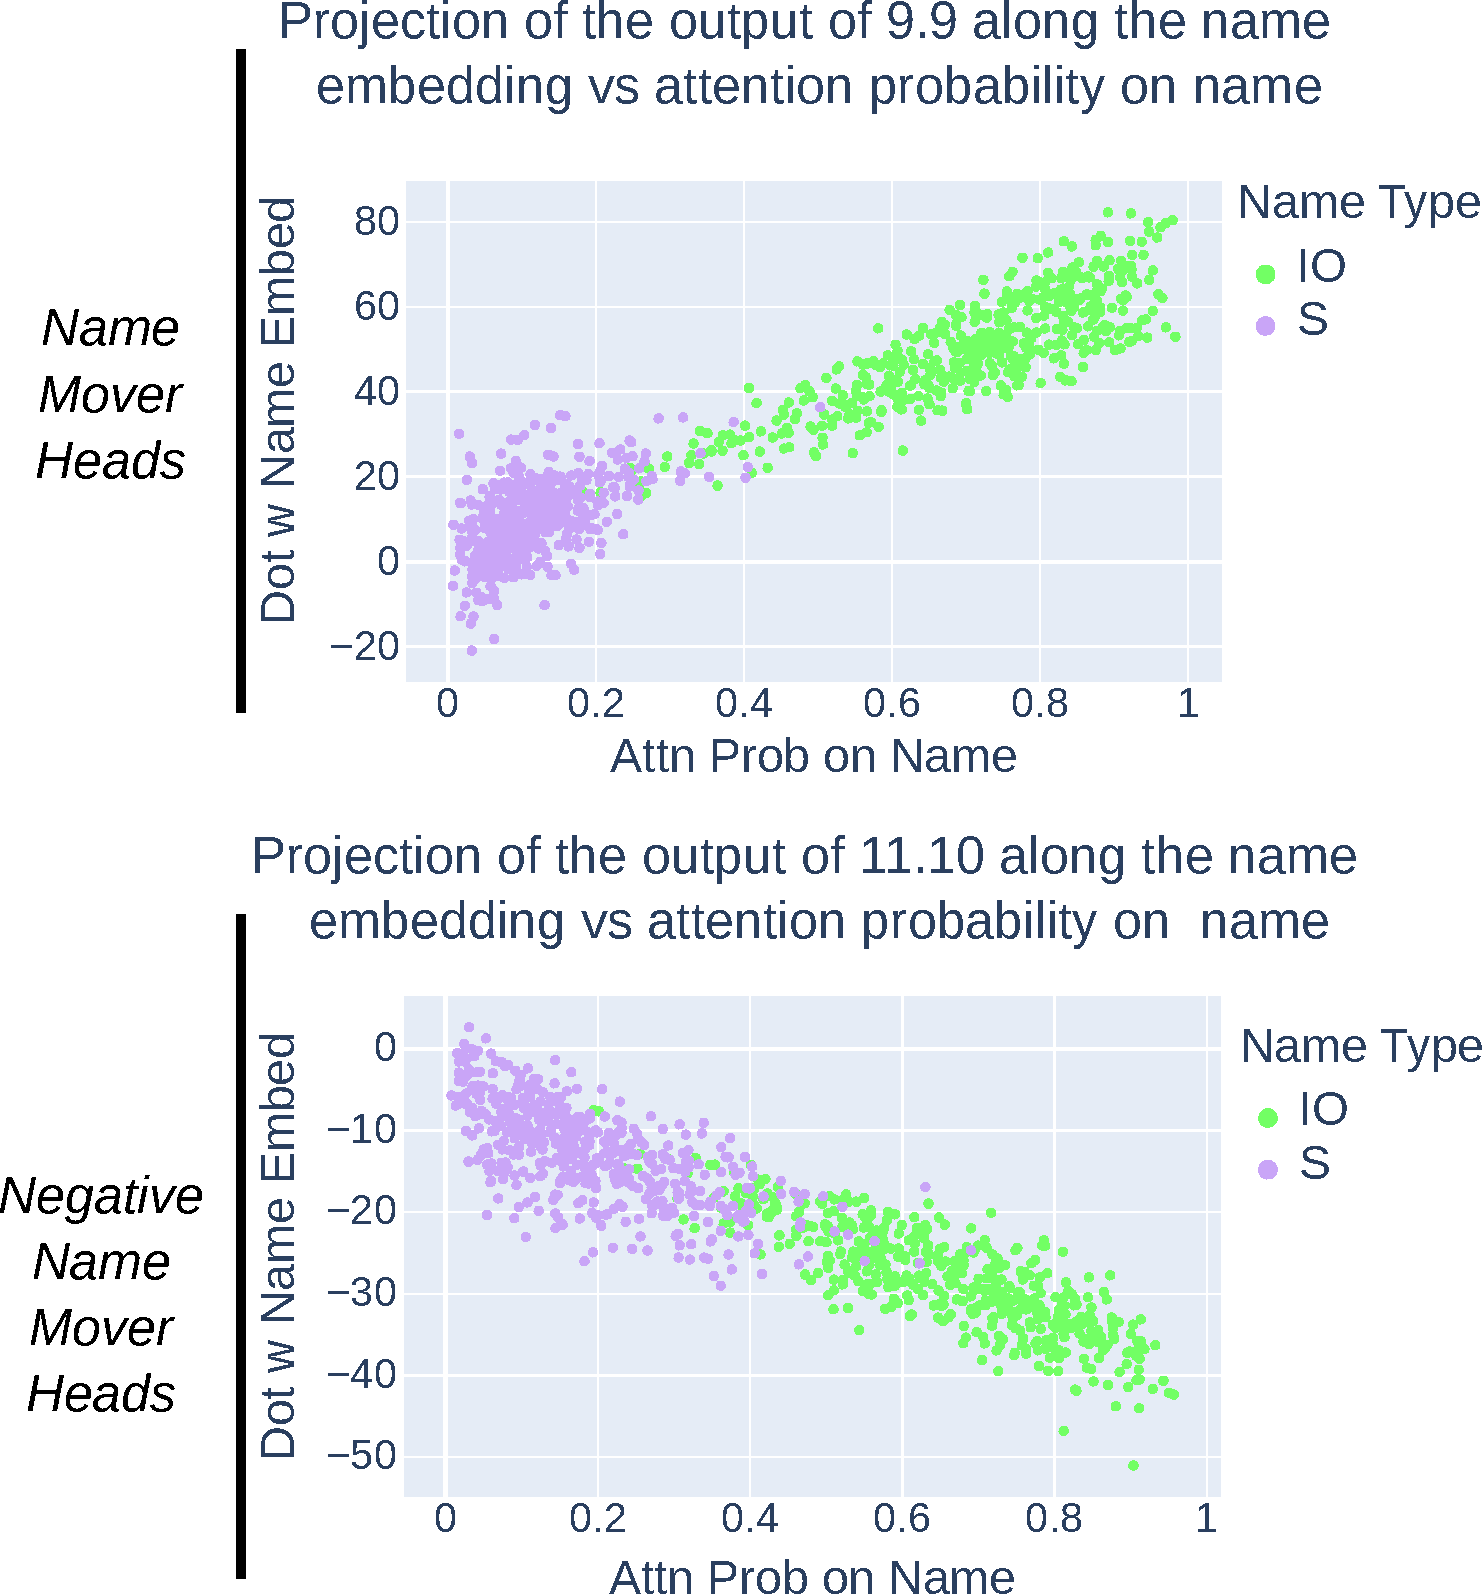
\includegraphics[width=\textwidth]{figs/fig_nm_neg_legibilityB.pdf}
         \caption{}
         \label{fig:name_moversC}
     \end{subfigure}
     \hfill
    \caption{(a) We are searching for heads $h$ directly affecting the logits using path patching. (b) Results of the path patching experiments. Name Movers and Negative Name Movers Heads are the heads that have the strongest direct effect on the logit difference. (c) Attention probability vs projection of the head output along $W_{U}[IO]$ or $W_{U}[S]$ respectively. For S tokens, we sum the attention probability on both S1 and S2. }%(c) Value-weighted attention score with the query at the end token. (d) Top: copying score for the Name Mover Heads, bottom: negative copying score for the Negative Name Mover Heads. Dashed lines are the average scores for all heads.}
    \label{fig:name_movers}
\end{figure}


% Their discovery was a surprise to us. It's not clear what role do they play, we hypothesize that they act as calibration. Even if IO is the most likely answer, language models are trained to predict an accurate probability distributions such that IO should not have 100\% probability. The negative heads could refine the estimate of previous heads to limit overconfident estimations.

\subsection{Which heads affect the Name Mover Heads' attention? (S-Inhibition Heads)}
\label{sec:s_inhibition}

\textbf{Tracing back the information flow.} Given that the Name Mover Heads are primarily responsible for constructing the output, we next ask what heads they depend on. As illustrated in Figure~\ref{fig:sinA}, there are three ways to influence attention heads: by their values, keys, or queries. In the case of Name Mover Heads, their value matrix appears to copy the input tokens (see previous section), so we do not study it further. Moreover, as the IO token appears early in the context, the Name Mover Heads' key vectors for this position likely do not contain much task-specific information. Therefore, we focus on the query vector, which is located at the END position. 

We again use path patching, identifying the heads that affect each Name Mover Head's query vector. Specifically, for a head $h$ we patch the path $h \to \text{Name Mover Heads' queries}$ (Figure~\ref{fig:sinA}) and report the effect on logit difference in Figure~\ref{fig:sinB}. %quantify the direct effect of each head on the queries of Name Movers Heads by performing path patching. We freeze every heads on the path from the output of the patched head $h$ at the END position, to the queries of the Name Mover Heads. We then measure the indirect effect on the logit difference (the Name Mover Heads and later heads are not frozen). See Figure \ref{fig:sinA} for an illustration of the experiment. 
%
%The results of this experiment are shown in Figure \ref{fig:sinB}. 
Heads 7.3, 7.9, 8.6, 8.10 directly influence the Name Mover Heads' queries, causing a significant drop in logit difference through this path. 

\textbf{S-Inhibition Heads.} To better understand the influence of these heads on the Name Movers Heads, we visualized Name Movers Heads' attention before and after applying path patching of all four previously identified heads at once (Figure \ref{fig:sinC}). Patching these heads leads to a greater probability on S1 (and thus less on IO). We therefore call these heads \emph{S-Inhibition Heads}, since their effect is to decrease attention to S1.
%Patching decreases attention to the IO token, indicating that these heads are counterfactually important for the Name Mover Heads's specific attention on the IO token on $\pioi$, compared to the CDE distribution. We call these newly identified heads \textbf{S-Inhibition Heads}, because in $\pioi$ they primarily cause the Name Mover Head attention to drop on the S tokens (thus increasing the attention on the IO token).


\begin{figure}
    \centering
     \begin{subfigure}[b]{0.3\textwidth}
         \centering
         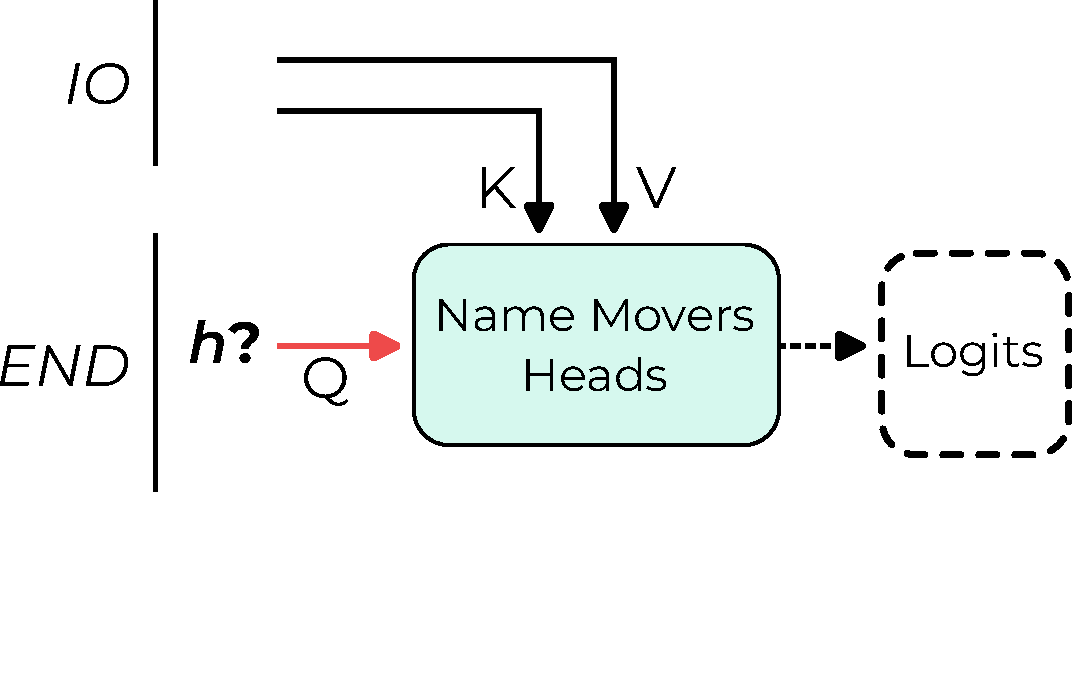
\includegraphics[width=\textwidth]{figs/sinA.pdf}
         \caption{}
         \label{fig:sinA}
     \end{subfigure}
     \hfill
     \begin{subfigure}[b]{0.30\textwidth}
         \centering
         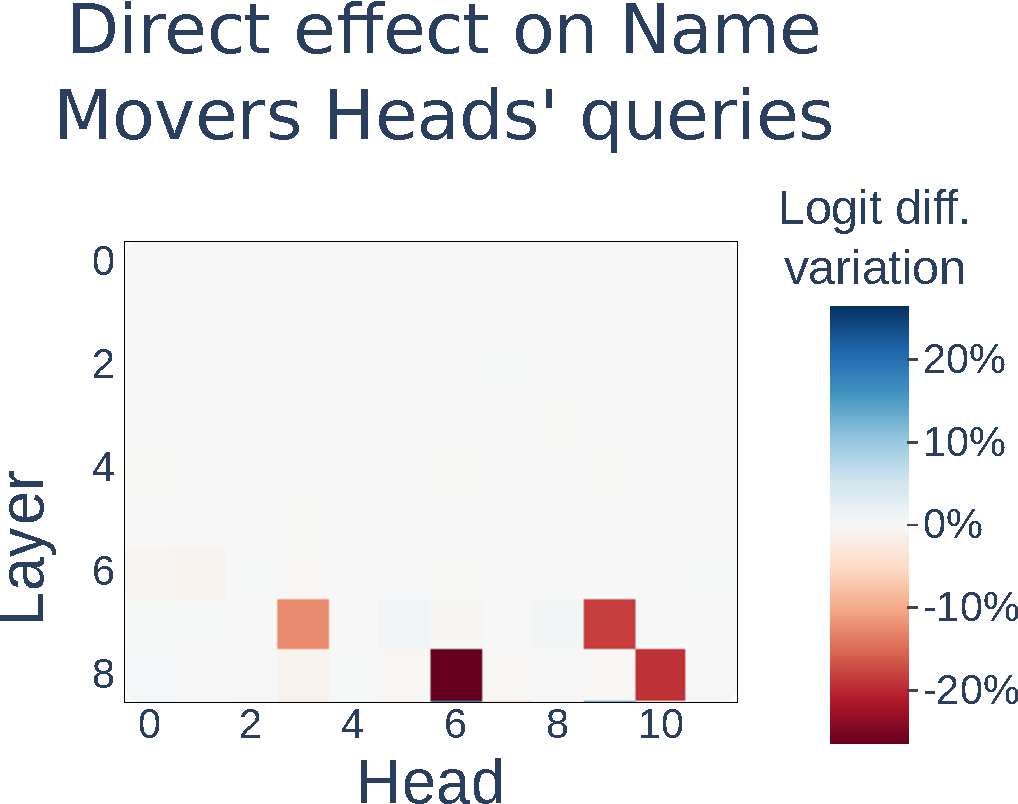
\includegraphics[width=\textwidth]{figs/sinB.pdf}
         \caption{}
         \label{fig:sinB}
     \end{subfigure}
     \hfill
     \begin{subfigure}[b]{0.35\textwidth}
         \centering
         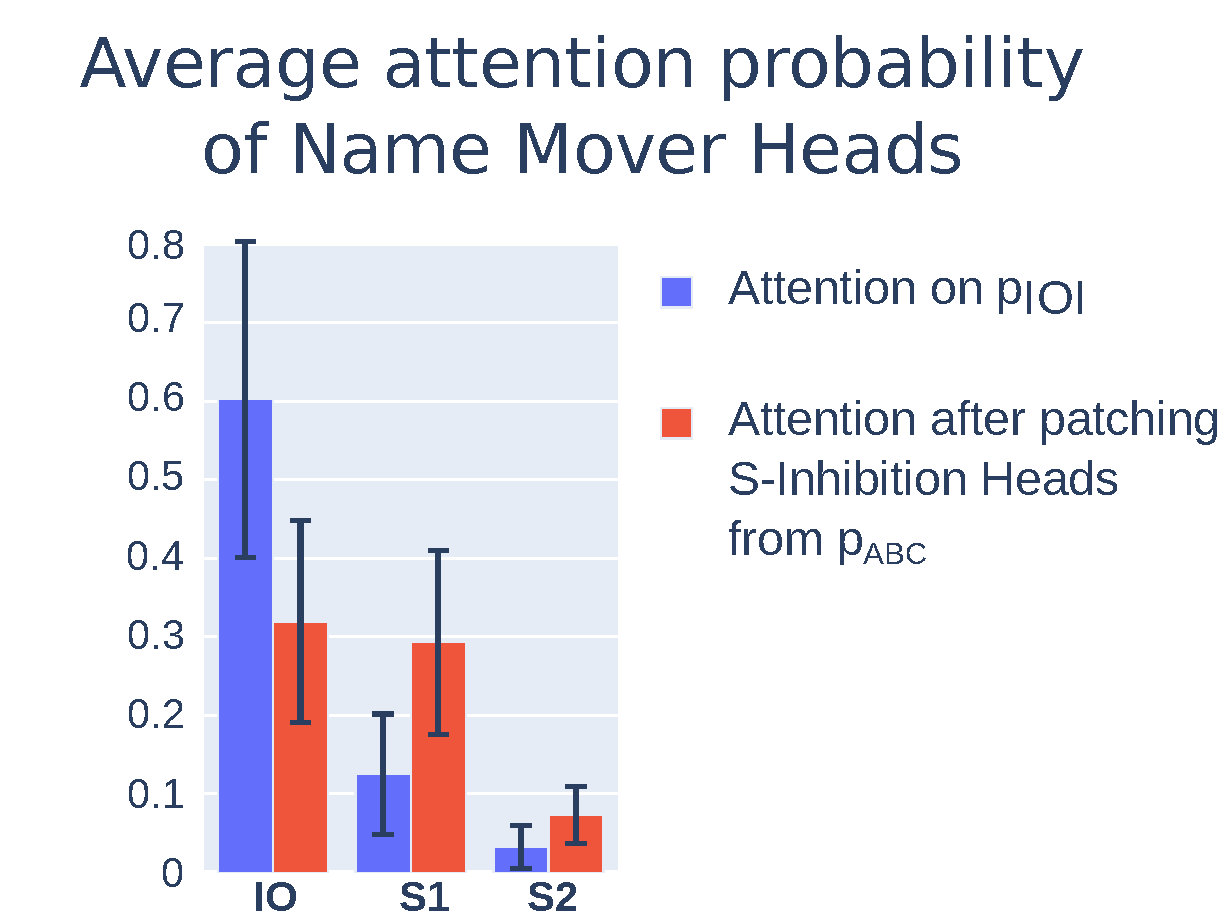
\includegraphics[width=\textwidth]{figs/sinC.pdf}
         \caption{}
         \label{fig:sinC}
     \end{subfigure}
    \caption{(a) Diagram of the direct effect experiments on Name Mover Heads' queries. We patch in the red path from the $\pabc$ distribution. Then, we measure the indirect effect of $h$ on the logits (dotted line). All attention heads are recomputed on this path. (b) Result of the path patching experiments. The four heads causing a decrease in logit difference are S-Inhibition Heads. (c) Attention of Name Mover Heads on $\pioi$ before and after path patching of S-Inhibition Heads $\to$ Name Mover Heads' queries for all four S-Inhibition Heads at once (black bars show the standard deviation). S-Inhibition Heads are responsible for Name Mover Heads' selective attention on IO.}
    \label{fig:sin}
\end{figure}


%causes a decrease in the attention probability on IO, indicating that they are counterfactually important for the Name Mover Heads's attention probability on the IO token. 
%what has changed from the ABC distribution to the pIOI distribution to cause the Name Mover Heads to attend to the IO token preferentially?

%There are three ways to influence an attention heads:  

%these Name Mover Heads pay preferential attention to the IO token.

%Given that the Name Mover Heads are primarily responsible for constructing the output, we ask why these Name Mover Heads pay preferential attention to the IO token. There are two ways to affect the Name Mover Heads's attention: through the query vector at the END token or the key vector at the IO token. Since the key vector appears early in the context, it likely does not contain much task-specific information, so we focus on the END query vector. 

%By investigating Name Mover Heads on the ABC distribution (where all three names in the input are distinct; see Section~\ref{sec:knockouts}), we observed that their attention is not selective: they pay equal attention to the first two names. We thus ask: what has changed from the ABC distribution to $\pioi$ to cause the Name Mover Heads to attend to the IO token preferentially? 

% ARTHUR REWRITES AS NEXT PARA
% To empirically answer this question, we perform a \emph{patching} experiment. 
% %\footnote{Our technique is similar to causal tracing from \cite{meng2022locating} or the interchange intervrentions from \cite{geiger2021causal}.}. 
% As illustrated in Figure \ref{fig:directed_graph_figure}, this technique consists of two steps. First, we save all activations of the network run on a source sequence. Then, we run the network on a target sequence, replacing some activations with the activations from the source sequence. We can then measure the behavior of the patched model. Doing this for each node individually locates the nodes that explain why model behavior is different in the source and target sequences. 
% END OF REWRITES

%To answer this question, we introduce patching experiments (Figure \ref{fig:directed_graph_figure}) used here and in the next section (\ref{sec:s_inhibition2}). In the general case, patching consist of three steps. First, we save the activations from the model run on source sentences. Second, we perform several runs of the model on the target sentences, replacing (patching) the activations of different model components with the activations from the source sentences. Thirdly, we run the model on the target sentences without patching. These steps are used to compare a statistic about activations on the second runs with the third runs.

%In this case, for a given attention head, we first run activation patching with source sentences from the ABC distribution. Then, we patch the activation of the attention head in the model running on target sentences from $\pioi$. Finally, we compute the change in attention probability from END to IO, averaged over the three Name Mover Heads. We do this for every head before layer 9 (the layer of the first Name Mover Head).

%To interpret the results, we first note that the Name Mover Heads attend more to IO in sequences from $\pioi$ than from ABC. If a head is important for Name Mover Heads selective attention on IO in inputs from $\pioi$, patching it from ABC to $\pioi$ should decrease how much Name Mover Heads attend on IO. The results from patching every head at the END token position are shown in Figure \ref{fig:new_just_patching}, right. We observe that patching heads 7.3, 7.9, 8.6, 8.10 causes a decrease in the attention probability on IO, indicating that they are counterfactually important for the Name Mover Heads's attention probability on the IO token. We call these heads \textbf{S-Inhibition Heads}, because in $\pioi$ they primarily cause the Name Mover Head attention to drop on the S tokens (thus increasing the attention on the IO token)


%In this case, we run activation patching with source distribution sentences from the ABC distribution and target distribution sentences from $\pioi$. Each sentence in the source distribution is a copy of the sentence in the target distribution, except S2 has been replaced by a random name. Running the model on the target distribution is the first step of the patching experiment. For the second step, we do runs where we patch in the target activations at the END position for each attention head except the Name Movers (Figure \ref{fig:new_just_patching}, right). We complete a run on the target distribution (the third step) so we can measure the counterfactual change in the Name Mover heads' attention to IO after patching, and find that the heads 7.3, 7.9, 8.6, 8.10 cause the largest attention decrease. We call these heads \textbf{S-Inhibition Heads}.

% remains of paragraph that AC rewrote
% We then compute the change in attention probability from END to IO, averaged over the three Name Mover Heads. We first note that the Name Mover Heads attends more to IO in input from $\pioi$ than from ABC. If a head is important for Name Mover Heads selective attention on $\pioi$, patching it from ABC to $\pioi$ should decrease how much Name Mover Heads attend on IO. The results from patching every head at the END token position are shown in Figure \ref{fig:new_just_patching}, right. We observe that patching heads 7.3, 7.9, 8.6, 8.10 causes a decrease in the attention probability on IO, indicating that they are counterfactually important for the Name Mover Heads's attention probability on the IO token. We call these heads \textbf{S-Inhibition Heads}, because in $\pioi$ they primarily cause the Name Mover Head attention to drop on the S tokens (thus increasing the attention on the IO token).% \todo{update figure to reflect this sentence}





\begin{figure}
    \centering
     \begin{subfigure}[b]{0.43\textwidth}
         \centering
         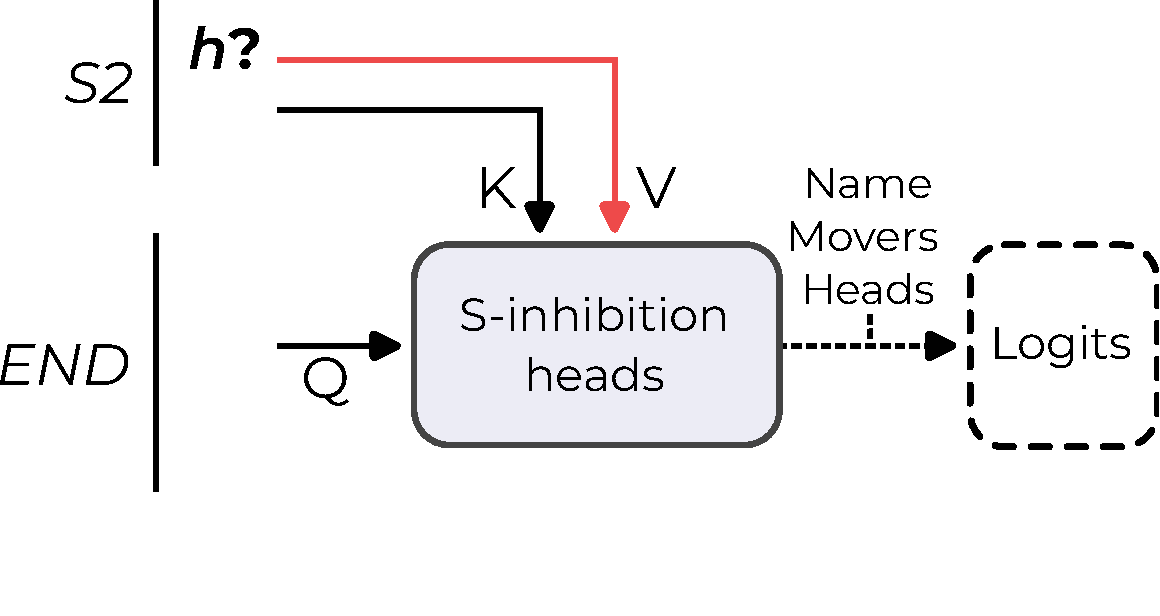
\includegraphics[width=\textwidth]{figs/Direct_effect_on_sinA.pdf}
         \caption{}
         \label{fig:effect_on_sinA}
     \end{subfigure}
     \hfill
     \begin{subfigure}[b]{0.43\textwidth}
         \centering
         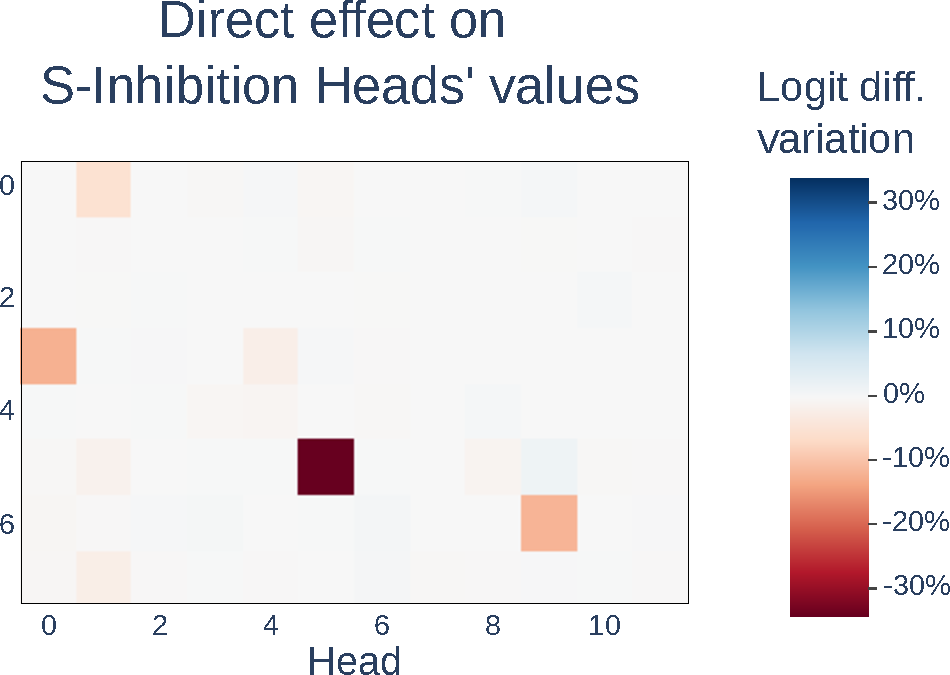
\includegraphics[width=\textwidth]{figs/Direct_effect_on_sinB.pdf}
         \caption{}
         \label{fig:effect_on_sinB}
     \end{subfigure}
    \caption{(a) Diagram of the direct effect experiment on S-Inhibition Heads' values. On the indirect path from $h$ to the logits (dotted line), all elements are recomputed, Name Movers Heads are mediating the effect on logits. (b) Result of the path patching experiments for the S-Inhibition Heads' values.}
    \label{fig:effect_on_sin}
\end{figure}


%\begin{figure*}
%    \centering
%    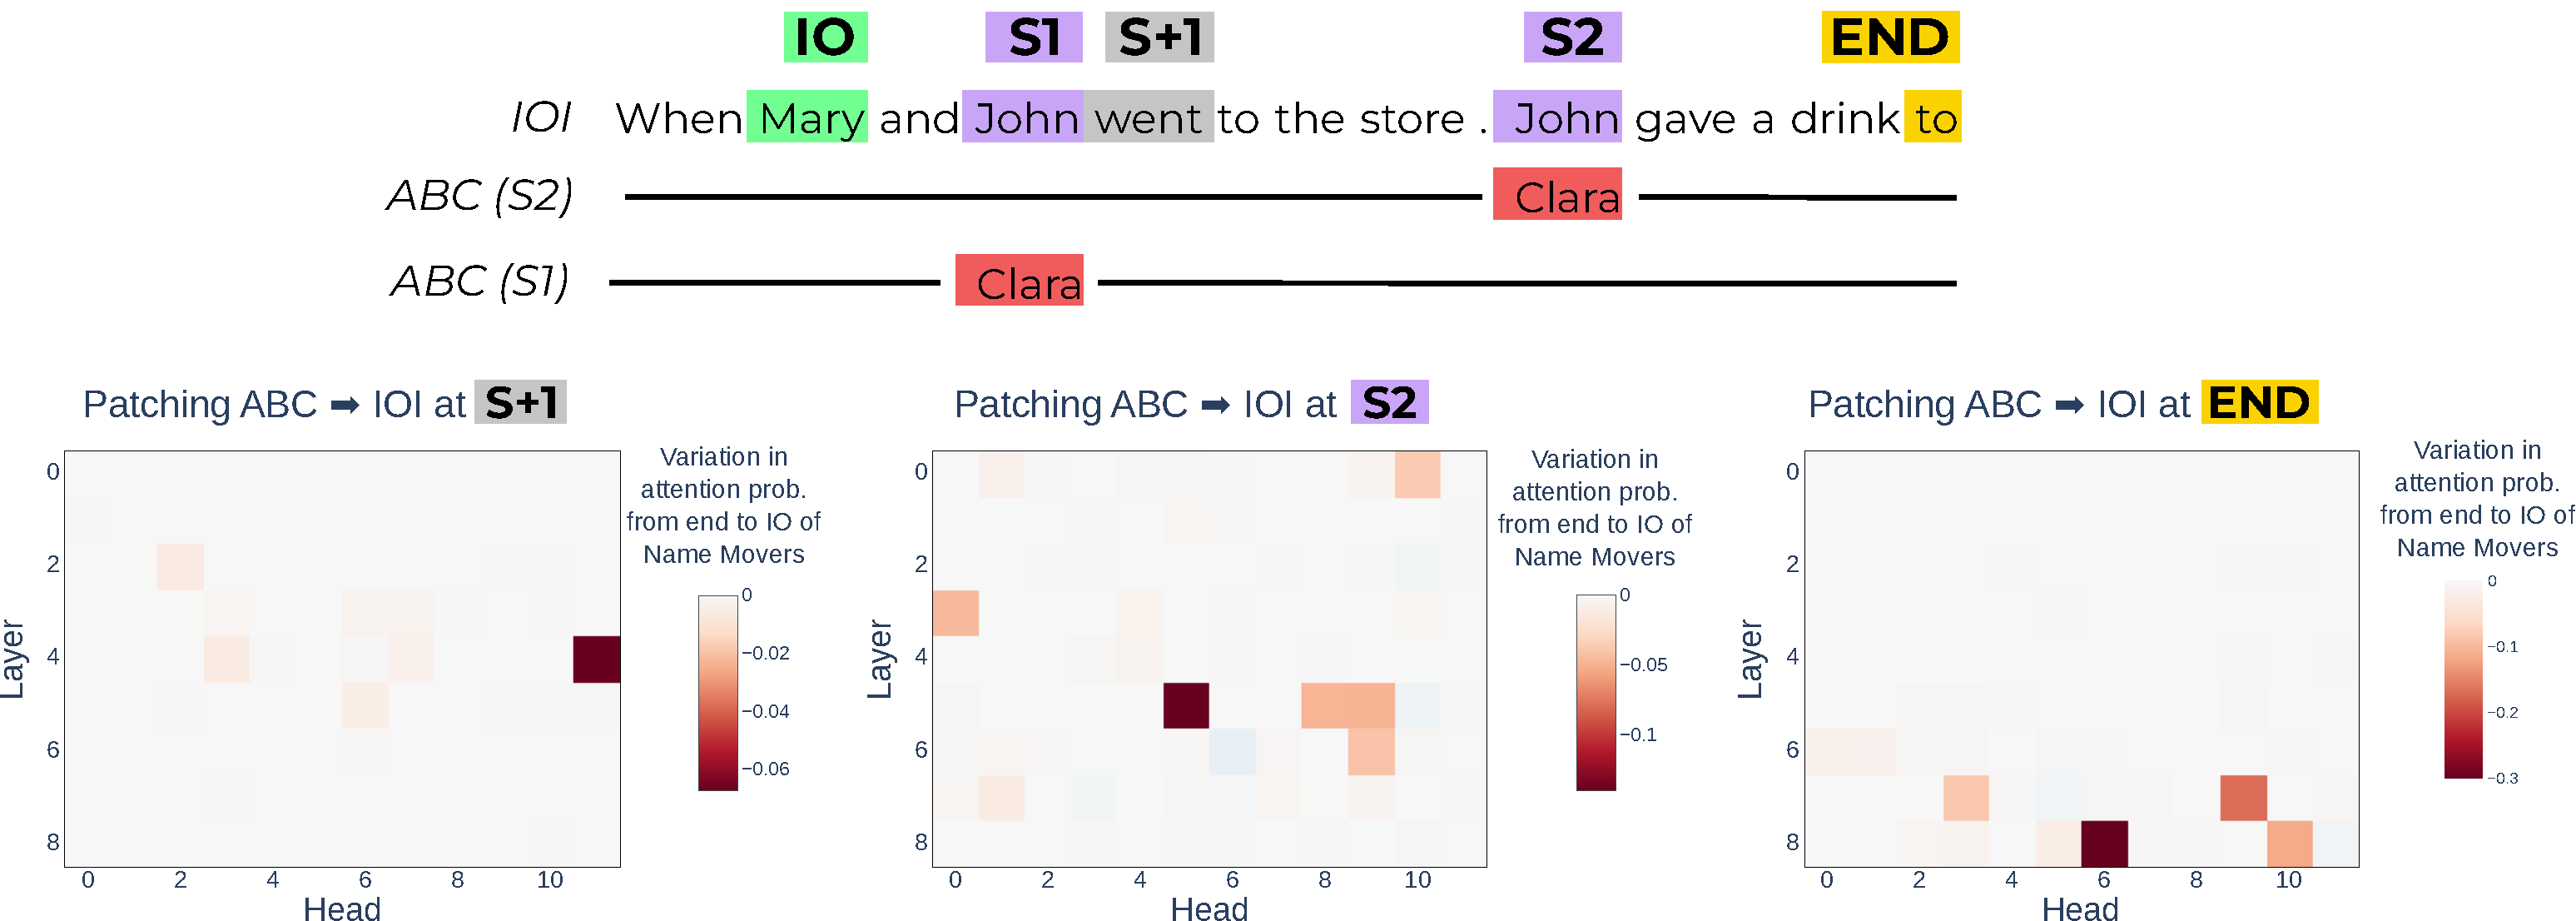
\includegraphics[width=\textwidth]{figs/patching_plots.pdf}
%    \caption{The attention probability to IO averaged over three Name Mover Heads is decreased most by the Previous Token Heads (left), Induction Heads (center) and S-Inhibition Heads (right) when we patch these attention heads from a sentence with a different S2 name (center and right), or a different S1 name (left). \todo{redo with new plots. Probably also mention CDE rather than ABC S1 etc}}
%    \label{fig:new_just_patching}
%\end{figure*}

\textbf{What are S-Inhibition heads writing?}
We observed that S-Inhibition heads preferentially attend to the S2 token (the average attention from END to S2 was 0.51 over the four heads). We conjectured that they move information about S that causes Name Movers to attend less to S1. We discovered two signals through which S-Inhibition Heads do this. The first, the \emph{token signal}, contains the value of the token S and causes Name Mover Heads to avoid occurrences of that token. The second, the \emph{position signal}, contains information about the position of the S1 token, causing Name Mover Heads to avoid the S1 position no matter the value of the token at this position.

To disentangle the two effects, we designed a series of counterfactual experiments where only some signals are present, and the others are inverted with respect to the original dataset (see Appendix~\ref{app:disantangling_signals}). 
%We quantified the effect of each signal by path patching the output of S-Inhibition Heads from these signal-specific datasets. 
Both effects matter, but position signals have a greater effect than token signals. These two signals suffice to account for the full average difference in Name Mover Heads' attention to IO over S1.
%A more detailed presentation of these experiments and their results can be found in Appendix \ref{app:disantangling_signals}.

S-Inhibition heads output information about the position of S1 but don't attend to it directly. They thus must rely on the output of other heads through value composition, as we will see next.

\subsection{Which heads affect S-Inhibition values?}
\label{sec:s_inhibition2}

\textbf{Tracing back the information flow.} We next trace the information flow back through the queries, keys, and values of the S-Inhibition Heads, using path patching as before. We found the values were the most important and so focus on them here, with keys discussed in Appendix~\ref{app:s_in_keys} (queries had no significant direct effect on the S-Inhibition Heads).

In more detail, for each head $h$ at the S2 position we patched in the path $h \to \text{S-Inhibition Heads's values}$ (Figure~\ref{fig:effect_on_sinA}) and reported results in Figure~\ref{fig:effect_on_sinB}. 

We identified 4 heads with a significant negative effect on logit difference.
By looking at their attention pattern, we separated them into two groups. The heads from the first group attend from S2 to S1, while those from the second group attend from S2 to the token after S1 (S1+1 in short). %We call them Induction-like Heads.

%S-Inhibition Heads attend primarily to S2 both on the IOI dataset (0.51 average attention) and on the CDE dataset (0.29 average attention). As the difference in attention is small, we don't expect Q or K path to be the most important here. For exhaustiveness, we conducted path patching experiments for all three inputs to the S-Inhibition Heads: queries, keys and values. We found heads causing the most important variation (30\% of the total logit difference) through the values of S-Inhibition Heads. We also found a significant effect size (6\% of the total logit difference) for the direct effect on the keys. The results of these two experiments are shown in Figure \ref{fig:effect_on_sin}.

%\textbf{Direct influence on S-Inhibition values.} We begin by describing the set of heads influencing logit difference through the values of S-Inhibition heads (Figure \ref{fig:effect_on_sinB}). By looking at their attention pattern, we separated them into two groups. The heads from the first group attend from S2 to S1, we call them Duplicate Token Heads. The heads from the second group attend from S2 to the token after S1, S1+1 in short. We call them Induction Heads.


% \textbf{Direct influence on S-Inhibition keys.} Due to space constraints, we describe the results of the direct effect through S-Inhibition Heads' keys, which has lower effect size than the value composition just discussed, in Appendix \ref{app:s_in_keys}. In short, we discovered three heads similar to the Induction and Duplicate Token Heads described above, but with less interpretable attention patterns. We called them fuzzy Induction Heads and fuzzy Duplicate Token Heads.

%To better understand how these heads behave, we characterize in more detail these two groups of heads.

%The next question to ask is: 

%How do the S-Inhibition Heads differentiate between IO and S, so they inhibit one but not the other? We measured their attention pattern and found that they preferentially attend to the S2 token (average attention to S2 at end 0.51 over all S-Inhibition heads). 
%Unfortunately, explaining this attention pattern proved intractable, which we elaborate on in Appendix \ref{app:S2 attention}. 
%We therefore studied what information these heads %S Inhibition heads
%move from the S2 token position to the END position. 

%To this end, we performed an identical patching experiment to that described at the end of Section \ref{sec:s_inhibition2}, except patching at the S2 position rather than the END position. We previously identified that S-Inhibition Heads attend to S2 and are also the only heads influencing Name Mover Heads at the END position. If the output of a head at S2 is copied by S-Inhibition Heads and later influences Name Movers Heads, it will be revealed by patching at S2. The results of this experiment are in Figure \ref{fig:new_just_patching}, center: a new sparse group of heads decreases the Name Movers Heads' attention probability on IO. We separate these into two classes based on their attention patterns: we call heads 6.9, 5.5, 5.8 and 5.9 Induction Heads, and 0.1, 0.10 and 3.0 Duplicate Token Heads.


%ALEX COMMENTED OUT
%We performed an identical patching experiment to that described at the end of Section \ref{sec:s_inhibition2}, except patching at the S2 position rather than the END position will reveal \ac{if that is whay we're trying to find out why don't we do it?} which heads are responsible for the S2 Inhibition heads' attention to S2. \av{This is *not* what these experiment are about: we try to see what information is copied by s-inhibition head} The results are in Figure \ref{fig:new_just_patching}, center: a new sparse group of heads decrease the attention probability on IO rather than S. We separate these into two classes based on their attention patterns: we call heads 6.9, 5.5, 5.8 and 5.9 Induction Heads, and 0.1, 0.10 and 3.0 Duplicate Token Heads.
% END ALEX COMMENT


% ARTHUR COMMENTED OUT
% To this end, we modified the information present at S2 and measure the variation in the Name Mover attention. 
% Towards this end, we ran a patching experiment at S2 from the ABC distribution to the IOI distribution and measured the variation in Name Mover Heads' attention. The results (Figure \ref{fig:new_just_patching}, center) reveal a large set of heads influencing Name Mover Heads' attention that did not appear at the END position. Logically, S-Inhibition Heads mediate this effect, as they are the only heads influencing Name Mover Heads at the END position. This reasoning suggests that the outputs of this set of head is moved by S-Inhibition Heads from S2 to the END token. When we analyze the attention patterns of these heads, we see two distinct groups emerge.
% END ARTHUR COMMENT

\textbf{Duplicate Token Heads.} Two of the heads attend from S2 to S1. We hypothesize that these heads attend to the previous occurrence of a duplicate token and copy the position of this previous occurrence to the current position. We therefore call them \emph{Duplicate Token Heads}.

% To rigorously test this hypothesis, we would study in details the interaction of the QK matrix with the token embeddings to test if it acts as a collision detector. Moreover, we would investigate the OV matrix to ensure it is copying information from positional embeddings. 

% Nonetheless, due to time constraint, 
To partially validate this hypothesis, we investigated these heads' attention patterns %outside $\pioi$. We analyze their attention pattern 
on sequences of random tokens (with no semantic meaning). We found that the 2 Duplicate Token Heads pay strong attention to a previous occurrence of the current token when it exists (see Appendix \ref{app:validation_dups}). 
%


% \todo{duplicate token heads and induction heads write binary signals instead of name information}

%Alexandre: I found this paragraph more confising that the original one, might come back to the previous one

\textbf{Induction Heads and Previous Token Heads.} The other group of two heads attends from S2 to S1+1. This matches the attention pattern of \emph{Induction Heads} \citep{elhage2021mathematical}, which recognize the general pattern \texttt{[A]\,[B]\,...\,[A]} and contribute to predicting \texttt{[B]} as the next token. For this, they act in pairs with Previous Token Heads. The Previous Token Heads write information about \texttt{[A]} into the residual stream at \texttt{[B]}. Induction Heads can then match the next occurrence of \texttt{[A]} to that position (and subsequently copy \texttt{[B]} to the output).
%token by reading the output of the Previous Token Head on \texttt{[B]}. It'll then copy the \texttt{[B]} token to the second \texttt{[A]} residual stream.

To test the hypothesis that this group of heads consists of Induction Heads, we sought out the Previous Token Heads that they rely on through key composition. To this end, we apply path patching to find heads that influence logit difference through the S1+1 keys of the Induction Heads (see Appendix \ref{app:prev_token_heads}). We identified two heads with significant effect sizes. 
To test the induction mechanism, we followed the method introduced in \citet{olsson2022context} by checking for prefix-matching (attending to \texttt{[B]} on pattern like \texttt{[A]\,[B]\,...\,[A]}) and copying (increasing the logit of the \texttt{[B]} token) of Induction Heads on repeated random sequences of tokens. We also analyzed the attention patterns of Previous Token Heads on the same dataset. As reported in Appendix~\ref{app:random_tok_seq}, Previous Token Heads attend primarily to the previous token and 2 Induction Heads demonstrate both prefix-matching and copying.

%However, we did not perform the more thorough parameter analysis presented in \cite{elhage2021mathematical} to validate at the parameter level the copying properties and key composition of Induction and Previous Token Heads.

%On repeated random sequences of tokens, we found that all the Previous Token Heads attend primarily to the previous token and the 2 Induction Heads demonstrate the prefix-matching and copying property (Appendix \ref{app:random_tok_seq}). 
%However, we were not able to validate the role of the fuzzy Induction Heads. We hypothesized that they are involved in fuzzy \ac{} induction as described by \citep{olsson2022context}, making them harder to appear on these strict tests.

%we patched activations from a sentence where S1 is replaced by a random name, at the S1+1 token index. As shown in Figure \ref{fig:new_just_patching}, some heads (and particularly 4.11) appear to influence Name Mover Heads. Then, by looking at the attention pattern of the heads with the most important influence in this patching experiment, we identified 3 Previous Token Heads. After analyzing attention patterns on random token sequences, we found that 2 of the 3 Previous Token Heads and 2 of the 4 Induction Heads demonstrated the expected behavior in this out-of-distribution case (Appendix \ref{app:random_tok_seq}).

\textbf{Locating the position signal.} Despite their differences, the attention patterns of both groups of heads are determined by the position of S1, suggesting that their output could also contain this information. We thus hypothesized that Duplicate Token Heads and Induction Heads are the origin of the position signal described in Section~\ref{sec:s_inhibition}, which is then copied by S-Inhibition Heads. 

To test this hypothesis, we applied the same technique from the previous section to isolate token and position signals. We patched the output of the Induction and Duplicate Token Heads from sentences with altered position signals. We observed a drop in logit difference of almost the same size as patching the S-Inhibition Heads (at least 88\%). However, patching their output from a dataset with a different S1 and S2 token but at the same position doesn’t change the logit difference (less than 8\% of the drop induced by patching S-Inhibition Heads).


\textbf{Missing validations and caveats.} To fully validate the claimed function of the Duplicate Token and Induction Heads, we would want to perform additional checks that we omitted due to time constraints. First, for Duplicate Token Heads, we would want to study the interaction of the QK matrix with the token embeddings to test if it acts as a collision detector. Moreover, we would investigate the OV matrix to ensure it is copying information from positional embeddings.  For Induction Heads, we would perform the more thorough parameter analysis in \cite{elhage2021mathematical} to validate the copying and key composition properties at the parameter level.

Moreover, in the context we study, Induction Heads perform a different function compared to what was described in their original discovery. In our circuit, Induction Heads' outputs are used as positional signals for S-Inhibition values. We did not investigate how this mechanism was implemented. More work is needed to precisely characterize these newly discovered heads and understand how they differ from the original description of Induction Heads.


%In our task, the Induction Heads writing into the S2 residual stream is an additional way for S-Inhibition Heads to detect that S occurs earlier in the context, on top of the Duplicate Token Heads' role. These Induction Heads, like Duplicate Token Heads, appear to be interpreted by the latter part of the circuit as a flag signaling that S2 is duplicate.% (Appendix \ref{app:signal}). Add back latter after more evidence 


%We 
%We hypothesized that the group we 
%found evidence that this group indeed read from token position S1+1 due to Previous Token Heads, so we call them Induction Heads. This evidence comes from patching activations at the S1+1 token index from a sentence where S1 is replaced by a random name. As shown in figure \ref{fig:new_just_patching} this reveals a sparse set of new heads. 2.2, 2.9 and 4.11, three of the most important heads in this plot attended to the previous token on $\pioi$ \ac{do we have more evidence?}. 

%Duplicate Token Heads, Induction Heads and Previous Token Heads all contribute to the model's performance on the IOI task (section \ref{sec:validation}), and the causal interventions in the above show that on $\pioi$ at which token indices they matter. To check that our description of their roles at the token indices are correct, we subjected the classes to harder out-of-distribution tests of their duplication, induction and previous attending behaviors. We tested these behaviors on random tokens (Appendix \ref{app:random_tok_seq}) and 2 of the 3 Previous Token Heads, 2 out of 3 of the Duplicate Token Heads and 2 of the 4 Induction Heads passed these harder tests. % demonstrated the expected behavior in this out-of-distribution case (Appendix \ref{app:random_tok_seq}).



% We're unsure why the model has two different mechanisms to perform the same task.  %  Both mechanisms appear to end up using a similar mechanism for how they influence S2 Inhibition head behavior, however \todo{write the signal stuff}. %  Surprisingly, we see Induction Heads play a role that could've been done by Duplicate Token Heads alone.
% We find the specific group of heads that make induction heads possible by OWT mean ablating at the token position after S1 (S1 + 1), and we verify that 2.2, 2.9 and 4.11 which appear important in this ablation plot indeed pay attention to previous tokens.

% We found that 2 of the 3 Previous Token Heads and 2 of the 4 Induction Heads demonstrated the expected behavior on this out-of-distribution context (see appendix \ref{app:random_tok_seq} for more details). We hypothesized that the other heads play a similar role on meaningful sequences.

\subsection{Did we miss anything? The Story of the Backup Name Movers Heads}
\label{sec:distributed_name_movers}

% As demonstrated in \cite{AnthropicMechanisticEssay}, a single task can be fulfilled by several heads (for example, induction heads). This suggests that transformers circuits naturally tend to be redundant and distributed\footnote{It is unlikely that SGD selects for perfectly redundant modules, but it is possible to obtain partial redundancy or full redundancy on a specific dataset.}. This idea is also consistent with the structure observed in Figure \ref{fig:name_movers}: despite having characterized the main contributing heads, many other heads seem to be significantly writing along the $W_{U}[IO]- W_{U}[S]$ direction. 
% As visible in figure \ref{fig:minimality}, this group contains heads that aren't individually influential but matter in aggregate.

%Given that each main class in our circuit contains multiple heads, transformer internals seem to naturally tend towards redundant or distributed circuits. 
Each type of head in our circuit has many copies, suggesting that the model implements redundant behavior\footnote{It is unlikely that SGD would select for perfectly redundant modules, but redundancy is more likely when analyzing a sub-distribution of all of a model's training data or a subtask of its behavior.}. To make sure that we didn't miss any copies, we knocked out all the Name Mover Heads at once. To our surprise, the circuit still worked (only 5\% drop in logit difference). After the knockout, we found the new heads directly affecting the logits using the same path patching experiment from Section~\ref{sec:name_movers}. % (as introduced in Section \ref{sec:name_movers}). 
%We discovered a group of heads that contribute positively to the logit difference, significantly more than they did before the knockout. 
These new heads compensate for the loss of Name Movers Heads by replacing their role.

We selected the eight heads with the highest direct influence on logit difference after knockout and call them \emph{Backup Name Mover Heads}. We investigated their behavior before the knockout. We observe diverse behavior: 4 heads show a close resemblance to Name Mover Heads, 2 heads equally attend to IO and S and copy them, 1 head pays more attention to S1 and copies it, and 1 head seems to track and copy subjects of clauses, copying S2 in this case. See Appendix \ref{app:backup_name_movers} for further details on these heads.

We hypothesize that this compensation phenomenon is caused by the use of dropout during training. Thus, the model was optimized for robustness to dysfunctional parts. More work is needed to determine the origin of this phenomenon and if such compensation effects can be observed beyond our special case. 

% 

%that previously did not write in the IO-S direction do so after the knockout.

%We discover another such distributed mechanism, finding evidence for a compensation mechanism for the Name-Mover Heads. When we knock-out the Name-Mover Heads, we find a large set of heads writing in the $W_{U}[IO]- W_{U}[S]$ direction that did not previously. 


% \begin{compactitem}
%     \item 3 heads show close resemblance to Name Movers.
%     \item 4 heads equally attend to IO and S and copy them.
%     \item 1 head pays more attention to S1 and copies it.
%     \item 1 head seems to track and copy subjects of clauses, copying S2 in this case.
% \end{compactitem}
 %Despite the fact that some of these heads naturally write in the direction of $W_{U}[S]$ over $W_{U}[IO]$, they all write along $W_{U}[IO]- W_{U}[S]$ after knocking out the main Name-Movers, showing the existence of a compensation mechanism that is not yet understood. 

% The distinction between the heads that were chosen and the one we decided to ignore was made qualitatively, and we decided on an arbitrary threshold. However, those are also the heads with that individually have the least influence on the global behavior of the circuit. As such, they are not the crucial parts to understand. This class of node is the one we understand the least, and there are many phenomena still to explore to understand how exactly the IO token is written into the residual stream.

% \subsection{}

%OLD

%Figure 2 Caption OLD 
% We discover a circuit in GPT-2 small that implements an algorithm that can compute IOI. Attention heads in the final 3 layers, which we call Name Movers (NMs), copy names into the residual stream proportional to their attention pattern. When performing IOI, the NMs preferentially pay attention to the Indirect Object (IO) to push the IO as the correct model output. The Name Mover circuit is distributed: Negative Heads will copy the negative of the IO (for what we hypothesize are calibration reasons) and Distributed Name Mover Heads take on the role of the NMs when the NMs are knocked out. The main NMs pay preferential attention to the IO because of the S Inhibition Heads, named so because they inhibit Name Mover attention on the Subject (S) tokens. The S Inhibition Heads move information about the repeated S tokens written by two groups of heads. Duplicate Token Heads write a signal that conveys that the S token was repeated at the S2 token position. Induction Heads do the same through an induction mechanism, where Previous Token Heads write information about the S1 token at the S1 + 1 token position, which Induction Heads then pass along at the S2 token position.}


%In our circuit, attention heads in the final 3 layers, which we call Name Mover Heads, copy names into the residual stream proportional to how much attention they pay to the name in the context. In the IOI distribution, the Name Mover Heads preferentially pay attention to the IO token, pushing the IO token as the correct model output. 

%S Inhibition Heads cause the Name Mover Heads to pay less attention to the S tokens (S1 and S2) and more attention to the IO token, writing at the END position and reading from the S2 token position. 

%The S Inhibition Heads are reading information about the S1 and S2 tokens, written by Duplicate Token Heads, which write information about S1 and S2 at the S2 token position \ac{could be misinterpreted - the info doesn't contain anything about the literal token S1, it's just a signal that there is a repeated token}, and Induction Heads, which do the same through an induction mechanism.

%Our circuit does not explain the attention patterns of the heads, and does not include the Layer Norm or MLPs. 

% \begin{itemize}
%     \item \emph{Previous-Token Heads} are active at position $S1+1$, attend to token $S$, and copy the embedding of $S$ into the residual stream.
%     \item \emph{Induction Heads} are active at position $S2$, attend to token $S1+1$ (mediated by the Previous-Token head), and copy the $S1+1$ token into the residual stream. Curiously, these induction heads influence the $S$-inhibition heads: \emph{the fact that the induction heads are copying} is a signal that $S2$ appeared previously, and should therefore be inhibited.
%     \item Finally, \emph{Backup Name-Mover Heads} do not normally move the IO token to the output, but take on this role if the regular Name-Mover Heads are ablated. \todo{consistent capitalisation of `heads'}
% \end{itemize} 

%\textbf{Copying behavior.}
%As shown in figure \ref{fig:name_movers}, the the heads that write most strongly in the IO-S direction pay preferential attention to the IO token. The apparent linear relationship between attention paid and writing suggests that these heads are copying the token from the position they attend to. For this reason, we call heads with this behavior the Name Mover Heads (NMHs).

%In order to validate this hypothesis, we investigated the OV matrices of the NMHs in isolation. We considered a circuit where we only kept the first layer of the transformer, the matrix multiplication by $W_{OV}$ for one NMHs and the final LayerNorm and unembedding. On tokens representing names, this circuit is implementing the identity function: the most likely token is the token in input. This is not the default behavior, as most of the attention heads implement other processing in their OV circuit such that in the same setting, the current token in not present. The results of this experiment are presented in figure \ref{fig:name_movers}.

%activation patching s-inhibition
%We then do an activation patching experiment to causally confirm that these four heads are responsible for the NM attention pattern. Our source distribution is the ABC template distribution (where there are three random names) and our target distribution is the normal ABB distribution \todo{check that previous section leads into this well}. In the ABC distribution, the NM attention patterns are diffuse across all three names, and we assume that the heads that influence the attention patterns of the NMs are constant across both distributions and behave differently due to the difference in the inputs. Thus, patching from the ABB distribution to the ABC distribution will reveal which heads counterfactually cause the NMs to pay preferential attention to the IO in the ABB distribution while not in the ABC distribution. 



%We hypothesize that the mechanism that causes this preferential attention must compose with the NHMs' Query at the END token position because its keys are too early in the context to contain relevant information about the task. 
%Thus, as described in \ref{sec:methods}, we OWT mean ablate attention heads at the END index to discover important heads.

% The results are shown in Figure \ref{fig:s2_ablation_patch}, top right. We find four heads (7.3, 7.9, 8.6, 8.10) that show up strongly on these plots, causing a drop larger than that caused by the Name Mover Heads.

% If we inspect the attention pattern of the name-movers after ablating these heads, we see that it is more uniform over the three names: the attention on both S tokens increases. We therefore hypothesize that these heads inhibit attention to the S tokens, and so refer to them as \textit{S-Inhibitions Heads}. % are responsible for the Name Movers' preferential attention on IO.

% \begin{figure*}
% \centering
% 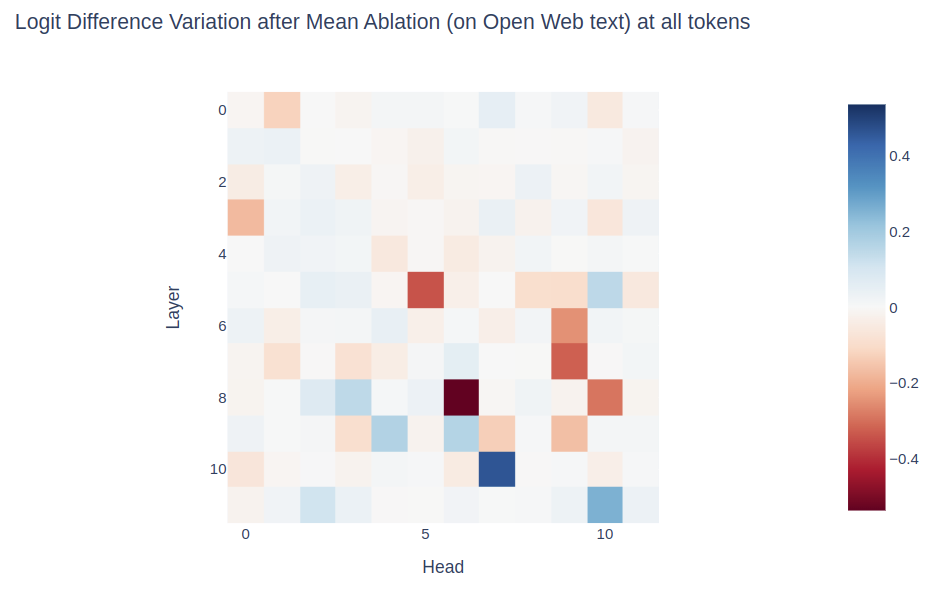
\includegraphics[width=0.4\textwidth]{figs/S2_INHIBITION_OWT.png}
% \caption{Plot of change logit difference metric when OWT knocking out different heads in the network.}
% \label{fig:s2_inhibition_ablations}
% \end{figure*}



% \subsubsection{Activation Patching}
% \label{sec:patching}
% In patching, we compute a forward pass of the network on a \texit{source} distribution, saving all activations computed. We then perform a forward pass on the \textit{target} distribution, replacing some activations with the activations from the source distribution. Activation patching can be viewed as an ablation where the dataset used to sample the activations from is different from the dataset we run the model on, and such a dataset may differ for each of the inputs in the batch of the source distribution. In practice, we use patching as a technique for causal interventions on models to verify or contradict hypotheses. 
%, unlike the attribution and removal use cases of ablation, and so the two serve different purposes.

% an ablation that only ablates directions that are specific to the target distribution. 

% To further investigate, we consider a counterfactual input with an ``ABC'' rather than ``ABB'' pattern of names (instead of \emph{John and Mary\ldots John gave}, we have \emph{John and Mary\ldots Charlie gave}). We first inspected the attention patterns of the name-mover heads on this ABC distribution, and observed that it is diffuse across all three names. 